\documentclass[a4paper,12pt]{ctexart}

\usepackage{tikz}% 画图用的包
\usepackage{graphicx} %插入图片的宏包
\usepackage{float} %设置图片浮动位置的宏包
\usepackage{subfigure} %插入多图时用子图显示的宏包
\usepackage{fancyhdr} %设置页眉页脚的宏包
\usepackage[]{caption2} %设置图和表的格式的宏包
\usepackage{multirow} %合并多行单元格的宏包
\usepackage{longtable} %不宽但很长的表格可以用longtable宏包来进行分页显示
\usepackage{array} %一般用于数学公式中对数组或矩阵的排版
\usepackage{makecell}% makecell命令对表格单元格中的数据进行一些变换的控制。我们可以使用 \ 命令进行换行,也可以使用p{(宽度)}选项控制列表的宽度
\usepackage{threeparttable} %制作三线表格
\usepackage{booktabs}%s三线表格中的上中下直线线型设置宏包,在这个包中水平线被教程\toprule、midrule、buttomrule。
\usepackage{enumerate} %列举宏包

% 以下是伪代码
\usepackage{algorithm}
\usepackage[noend]{algpseudocode}
\floatname{algorithm}{算法}


%页眉页脚设置
\pagenumbering{arabic}
\pagestyle{fancy}
\setlength{\headheight}{15pt}
\fancyhead[L]{\reportType}
\fancyhead[R]{\className \reportSemester}
\fancyhead[C]{}
\fancyfoot[C]{\thepage}

%标题序号长度设置
\setcounter{secnumdepth}{3}

%图片排版设置
\renewcommand{\figurename}{图} %重定义编号前缀词
\renewcommand{\captionlabeldelim}{.~} %重定义分隔符
 %\roman是罗马数字编号,\alph是默认的字母编号,\arabic是阿拉伯数字编号,可按需替换下一行的相应位置
\renewcommand{\thesubfigure}{(\roman{subfigure})}%此外,还可设置图编号显示格式,加括号或者不加括号
\makeatletter \renewcommand{\@thesubfigure}{\thesubfigure \space}%子图编号与名称的间隔设置
\renewcommand{\p@subfigure}{} \makeatother

%表头文字格式的详细设置
\renewcommand\theadset{\renewcommand\arraystretch{0.85}%
\setlength\extrarowheight{0pt}}%行距
\renewcommand\theadfont{\small}%字体
\renewcommand\theadalign{rt}%行列对齐
\renewcommand\theadgape{\Gape[0.5cm][2mm]}%上下垂直距离

\title{
  \begin{figure}[H]
    \centering
    \includegraphics[width=1\textwidth]{./img/university.png}
  \end{figure} 
  \vspace{3em}
  \huge \textbf{\reportName} \\ 
  \vspace{1em}
  \large \textbf{\className-\reportType}\\
  \vspace{5em}
  \large 学生姓名\hspace{0.7cm}\underline{\makebox[5.5cm]{\studentName}} \\
  \large 学生学号\hspace{0.7cm}\underline{\makebox[5.5cm]{\studentID}} \\
  \large 专业班级\hspace{0.7cm}\underline{\makebox[5.5cm]{\studentGrade}} \\
  \large 指导教师\hspace{0.7cm}\underline{\makebox[5.5cm]{\prof}} \\
  \large 提交日期\hspace{0.7cm}\underline{\makebox[5.5cm]{\the\year 年 \the\month 月 \the\day 日}} \\
}

\author{}
\date{}

\ctexset { section = { format={\Large \bfseries } } }


\usepackage{tikz} % 确保 TikZ 包被引入
\usetikzlibrary{shapes,arrows,automata} % TikZ 库,用于绘制状态图等
\usepackage{amssymb} % 添加数学符号支持
\usepackage{amsmath} % 添加更多数学支持
\usepackage{unicode-math} % 添加Unicode数学符号支持

\newcommand{\studentName}{xxx} % 学生姓名
\newcommand{\studentID}{xxxxxxx} % 学生学号
\newcommand{\studentGrade}{计算机科学与技术} % 学生班级

\newcommand{\reportName}{为什么P是否等于NP是计算机科学领域最重要的理论问题}
\newcommand{\className}{算法分析与设计}
\newcommand{\reportType}{课程报告}
\newcommand{\reportSemester}{2025春}
\newcommand{\prof}{杜嘉欣}


\begin{document}
\maketitle
\newpage


\section{内容与要求}
该课程报告假设你的读者是刚进入大一的同学,他们听说计算机学科最重要的问题是证明$P$是否等于$NP$。这些同学非常疑惑,为什么计算机学科终极问题不是计算而是这样一个证明。你需要在课程报告中向低年级的同学解答这一疑惑,为此你可以按照如下提纲撰写相关内容:
\begin{itemize}
    \item 计算机如何求解问题?
    \item 图灵机的原理是什么?
    \item 计算问题如何进行分类?
    \item 布尔可满足性问题(SAT)是$NP$完全问题吗?
    \item 旅行商问题(TSP)问题与SAT问题之间的关系是什么?
    \item 如果有人证明了$P$等于$NP$,对计算机学科将产生哪些影响?
\end{itemize}

课程报告的要求:
\begin{itemize}
    \item 课程报告要求独立完成,文字简练、合理分节、图文并茂,要求报告字数不少于1000;
    \item 阅读相关材料,并用自己的理解从新描述;
    \item 一旦与网上某个材料重复率超过20\%以上,将按抄袭处理;
    \item 详细列出参考的论文、网站。
\end{itemize}

\section{人们对可计算的探索:从希尔伯特之梦到计算的边界}
在计算机还未诞生的年代,人类对"计算"的思考早已开始。这种思考并非仅仅局限于数字的加减乘除,而是触及了更深层次的问题:哪些问题是"可解"的?是否存在一种通用的方法,可以判定任何数学命题的真伪?这个探索过程横跨了整个20世纪,涉及了数学、逻辑学和后来的计算机科学等多个领域,最终导致了现代计算理论的诞生。

\subsection{数学危机与希尔伯特纲领}
19世纪末到20世纪初,数学界经历了一场深刻的基础危机。这场危机源于集合论中发现的各种悖论,最著名的是罗素悖论:考虑"所有不包含自身的集合的集合",这个集合是否包含自身?无论答案是是还是否,都会导致矛盾。这些悖论的出现,动摇了人们对数学基础的信心。

在这样的背景下,希尔伯特提出了他的宏伟计划,试图通过以下步骤重建数学的基础:
\begin{enumerate}
    \item \textbf{形式化:} 将所有数学陈述形式化为一个精确的符号系统
    \item \textbf{完备性:} 证明这个系统是完备的,即任何陈述都能被证明或反驳
    \item \textbf{一致性:} 证明这个系统是一致的,即不会产生矛盾
    \item \textbf{可判定性:} 找到一个机械的过程,能够判定任何数学陈述的真伪
\end{enumerate}

希尔伯特在1900年巴黎国际数学家大会上提出的23个问题,成为了20世纪数学研究的重要指南。其中第二问题关注算术公理系统的一致性,第十问题则直接涉及算法的本质:是否存在一个通用算法,能够判定任意丢番图方程是否有整数解?

\subsection{希尔伯特的判定问题与哥德尔不完备性}
希尔伯特的"判定问题"(Entscheidungsproblem)是其数学纲领中最具挑战性的部分。这个问题可以形式化地表述为:是否存在一个机械化的过程(算法),能够对任意一阶逻辑公式,判定它是否是普遍有效的(在所有可能的解释下都为真)?

这个问题的重要性在于:
\begin{itemize}
    \item 如果存在这样的算法,就意味着所有数学问题原则上都是可解的
    \item 它迫使人们精确地定义什么是"机械化过程"或"算法"
    \item 它推动了可计算性理论的发展
\end{itemize}

然而,1931年,年仅25岁的奥地利数学家库尔特·哥德尔发表了震惊世界的不完备性定理。这个定理实际上包含两个密切相关的结果:

\textbf{第一不完备性定理:}
在任何包含基本算术的一致的形式系统中,存在既不能被证明也不能被反驳的命题。用现代的说法,这样的命题是"不可判定的"。这个定理的证明极其巧妙,哥德尔构造了一个自指的命题,大致相当于"这个命题不能在该系统中被证明"。如果这个命题能被证明,就会导致矛盾;如果它能被反驳,也会导致矛盾。因此,它必须是不可判定的。

\textbf{第二不完备性定理:}
任何足够强的形式系统都不能证明自身的一致性。这个结果直接打击了希尔伯特纲领的核心目标之一:用有限主义方法证明算术的一致性。

这两个定理的影响是深远的:
\begin{itemize}
    \item 表明数学中存在本质上不可判定的命题
    \item 证明了形式化数学系统的内在局限性
    \item 暗示了计算过程可能存在的根本限制
    \item 为后来的不可计算性理论奠定了基础
\end{itemize}

\subsection{计算模型的萌芽:多元化的探索}
在哥德尔的工作之后,数学家们开始寻找更具体的方式来刻画"机械过程"或"算法"的概念。这导致了多个不同但最终被证明等价的计算模型的提出:

\subsubsection{递归函数理论}
\begin{itemize}
    \item \textbf{原始递归函数:} 最基本的计算函数类,包括:
        \begin{itemize}
            \item 常数函数
            \item 后继函数
            \item 投影函数
            \item 复合运算
            \item 原始递归运算
        \end{itemize}
    \item \textbf{μ-递归函数:} 通过添加最小化算子,扩展了原始递归函数的能力
    \item \textbf{部分递归函数:} 允许函数在某些输入上不收敛,更接近实际的计算过程
\end{itemize}

\subsubsection{$\lambda$-演算}
邱奇的$\lambda$-演算是一个极其简洁但功能强大的计算模型:
\begin{itemize}
    \item \textbf{基本概念:}
        \begin{itemize}
            \item 变量:表示参数
            \item 抽象:定义函数
            \item 应用:函数调用
        \end{itemize}
    \item \textbf{主要特点:}
        \begin{itemize}
            \item 所有函数都是单参数的(多参数函数通过柯里化实现)
            \item 函数可以作为参数和返回值
            \item 没有显式的数据结构(一切都可以用函数编码)
        \end{itemize}
    \item \textbf{现代影响:}
        \begin{itemize}
            \item 函数式编程语言的理论基础
            \item 类型理论的发展
            \item 程序语言语义学的研究
        \end{itemize}
\end{itemize}

\subsubsection{图灵机}
图灵的方法与其他人不同,他试图模拟人类进行计算时的实际行为:
\begin{itemize}
    \item \textbf{设计思想:}
        \begin{itemize}
            \item 基于人类计算者使用纸笔进行计算的过程
            \item 将计算过程分解为最基本的步骤
            \item 强调计算的机械性和确定性
        \end{itemize}
    \item \textbf{创新之处:}
        \begin{itemize}
            \item 引入了无限存储的概念(纸带)
            \item 将计算状态与数据存储分离
            \item 提供了清晰的计算步骤定义
        \end{itemize}
\end{itemize}

\subsection{计算模型的统一:邱奇-图灵论题}
最令人惊讶的是,这些看似完全不同的计算模型最终被证明是等价的:
\begin{itemize}
    \item 任何图灵可计算的函数都是$\lambda$-可定义的
    \item 任何$\lambda$-可定义的函数都是递归的
    \item 任何递归函数都是图灵可计算的
\end{itemize}

这种等价性导致了邱奇-图灵论题的提出,它包含两个层面:
\begin{enumerate}
    \item \textbf{数学论题:} 上述所有计算模型定义的可计算函数类是相同的
    \item \textbf{物理论题:} 这个函数类恰好包含了所有直观上可计算的函数
\end{enumerate}

这个论题的重要性在于:
\begin{itemize}
    \item 为"算法"或"可计算性"提供了精确的数学定义
    \item 表明不同的计算方法本质上是等价的
    \item 暗示了计算能力可能存在普遍的上限
\end{itemize}

\subsection{从理论到实践:计算机的诞生与新问题的提出}
随着电子计算机的出现,理论研究的重点开始转向实际的计算效率问题:

\subsubsection{早期计算机的发展}
\begin{itemize}
    \item \textbf{机械计算时代:}
        \begin{itemize}
            \item 巴贝奇的差分机和分析机
            \item 霍勒瑞斯的打孔卡片机
            \item 机械计算器的普及
        \end{itemize}
    \item \textbf{电子计算机时代:}
        \begin{itemize}
            \item ENIAC的诞生
            \item 冯·诺依曼体系结构的提出
            \item 存储程序概念的确立
        \end{itemize}
\end{itemize}

\subsubsection{计算复杂性理论的兴起}
随着实际计算能力的提升,新的问题开始浮现:
\begin{itemize}
    \item \textbf{时间复杂性:}
        \begin{itemize}
            \item 算法运行时间的增长速度
            \item 多项式时间与指数时间的区别
            \item 最坏情况、平均情况和最好情况分析
        \end{itemize}
    \item \textbf{空间复杂性:}
        \begin{itemize}
            \item 存储空间需求的增长
            \item 时间-空间权衡
            \item 在线算法与离线算法
        \end{itemize}
    \item \textbf{复杂性类的研究:}
        \begin{itemize}
            \item P类问题的定义
            \item NP类问题的发现
            \item 复杂性层次的建立
        \end{itemize}
\end{itemize}

\subsection{现代计算理论的主要研究方向}
当代计算理论的研究已经远远超出了早期的范畴:

\subsubsection{算法设计与分析}
\begin{itemize}
    \item 近似算法的发展
    \item 随机算法的理论
    \item 量子算法的探索
\end{itemize}

\subsubsection{计算模型的扩展}
\begin{itemize}
    \item 并行计算模型
    \item 分布式计算理论
    \item 量子计算模型
\end{itemize}

\subsubsection{新兴研究领域}
\begin{itemize}
    \item 密码学理论
    \item 计算学习理论
    \item 算法博弈论
\end{itemize}

这些发展表明,计算理论不仅回答了"什么是可计算的"这个基本问题,还在不断探索"如何更好地计算"这个实践问题。P vs NP问题正是这两个方面的完美结合:它既是关于计算本质的深刻理论问题,也与实际的算法设计和应用密切相关。

\section{图灵机的原理:一切计算的理论基石}
图灵机是英国数学家艾伦·图灵在1936年发表的论文《论可计算数及其在判定问题上的应用》(On Computable Numbers, with an Application to the Entscheidungsproblem)中提出的一种抽象计算模型。它并非一台实体机器,而是一种思想实验工具,旨在精确定义"算法"或"机械过程"的概念。尽管图灵机结构异常简单,但它却拥有惊人的计算能力,能够模拟任何现代计算机(甚至未来可能出现的任何经典计算机)所能执行的计算过程。因此,图灵机成为了计算理论、可计算性理论和计算复杂性理论的奠基石。

\subsection{图灵的思考过程}
图灵提出这个模型时的思考过程非常有启发性:

\subsubsection{问题的提出}
图灵首先思考了这样一个问题:
\begin{itemize}
    \item 什么是"机械的"计算过程?
    \item 人类在进行计算时实际上在做什么?
    \item 如何将这个过程形式化?
\end{itemize}

\subsubsection{关键洞察}
通过观察人类计算者的行为,图灵得出了几个重要的洞察:
\begin{itemize}
    \item 计算过程可以分解为简单的、原子级的步骤
    \item 在任一时刻,计算者只能关注有限的信息
    \item 计算者需要某种外部存储来记录中间结果
    \item 计算者的行为是基于当前状态和观察到的符号
\end{itemize}

\subsection{图灵机的形式化定义}
一个图灵机可以形式化地定义为一个七元组 $M = (Q, \Gamma, b, \Sigma, \delta, q_0, F)$,其中:

\begin{itemize}
    \item $Q$:有限的状态集合
    \item $\Gamma$:有限的纸带字母表(包含所有可能出现在纸带上的符号)
    \item $b \in \Gamma$:空白符号
    \item $\Sigma \subseteq \Gamma \setminus \{b\}$:输入字母表
    \item $\delta: Q \times \Gamma \rightarrow Q \times \Gamma \times \{L,R\}$:转移函数
    \item $q_0 \in Q$:初始状态
    \item $F \subseteq Q$:接受状态集合
\end{itemize}

\subsection{图灵机的基本组成}
一个标准的图灵机由以下几个核心部分构成:

\subsubsection{无限纸带}
\begin{itemize}
    \item \textbf{物理特性:}
        \begin{itemize}
            \item 被划分为连续的单元格
            \item 向两端无限延伸
            \item 每个格子可以存储一个符号
            \item 初始时大部分格子包含空白符号
        \end{itemize}
    \item \textbf{实现考虑:}
        \begin{itemize}
            \item 实际实现时只需要分配用到的部分
            \item 可以用动态数据结构模拟
            \item 需要处理纸带扩展的情况
        \end{itemize}
    \item \textbf{存储特点:}
        \begin{itemize}
            \item 随机访问(通过移动读写头)
            \item 持久性(写入的内容保持不变直到被覆盖)
            \item 可重写(任何位置都可以被重写)
        \end{itemize}
\end{itemize}

\subsubsection{读写头}
\begin{itemize}
    \item \textbf{基本功能:}
        \begin{itemize}
            \item 读取当前格子的符号
            \item 写入新符号到当前格子
            \item 左右移动一个格子
        \end{itemize}
    \item \textbf{操作特点:}
        \begin{itemize}
            \item 原子性:每次操作都是不可分的
            \item 局部性:只能访问当前位置
            \item 顺序性:每次只能移动一格
        \end{itemize}
    \item \textbf{实现要求:}
        \begin{itemize}
            \item 需要维护当前位置信息
            \item 需要处理边界情况
            \item 需要确保操作的原子性
        \end{itemize}
\end{itemize}

\subsubsection{状态控制器}
\begin{itemize}
    \item \textbf{状态类型:}
        \begin{itemize}
            \item 初始状态:计算开始时的状态
            \item 工作状态:计算过程中的中间状态
            \item 接受状态:表示计算成功完成
            \item 拒绝状态:表示计算失败
        \end{itemize}
    \item \textbf{状态转换:}
        \begin{itemize}
            \item 基于当前状态和读取的符号
            \item 确定下一个状态
            \item 决定写入什么符号
            \item 决定读写头的移动方向
        \end{itemize}
    \item \textbf{设计考虑:}
        \begin{itemize}
            \item 状态数量要尽可能少
            \item 状态转换要清晰明确
            \item 避免死循环
        \end{itemize}
\end{itemize}

\subsection{图灵机的工作过程}
图灵机的计算过程可以分为以下几个阶段:

\subsubsection{初始化阶段}
\begin{itemize}
    \item \textbf{输入准备:}
        \begin{itemize}
            \item 将输入字符串写入纸带
            \item 其余格子填充空白符号
            \item 读写头定位到起始位置
        \end{itemize}
    \item \textbf{状态设置:}
        \begin{itemize}
            \item 将状态设为初始状态
            \item 准备转移函数表
            \item 确定停机条件
        \end{itemize}
\end{itemize}

\subsubsection{执行阶段}
\begin{itemize}
    \item \textbf{基本步骤:}
        \begin{enumerate}
            \item 读取当前格子的符号
            \item 根据当前状态和符号查找转移函数
            \item 执行转移函数指定的操作
            \item 检查是否达到停机状态
        \end{enumerate}
    \item \textbf{执行特点:}
        \begin{itemize}
            \item 确定性:相同输入产生相同输出
            \item 离散性:步骤是离散的
            \item 序列性:操作是顺序执行的
        \end{itemize}
\end{itemize}

\subsubsection{终止阶段}
\begin{itemize}
    \item \textbf{停机条件:}
        \begin{itemize}
            \item 达到接受状态
            \item 达到拒绝状态
            \item 无法继续执行(死循环)
        \end{itemize}
    \item \textbf{结果处理:}
        \begin{itemize}
            \item 确定计算是否成功
            \item 收集输出结果
            \item 释放资源
        \end{itemize}
\end{itemize}

\subsection{图灵机的变体与扩展}
\subsubsection{多带图灵机}
\begin{itemize}
    \item \textbf{结构特点:}
        \begin{itemize}
            \item 多个独立的纸带
            \item 每个纸带有自己的读写头
            \item 所有读写头同步移动
        \end{itemize}
    \item \textbf{计算能力:}
        \begin{itemize}
            \item 与单带图灵机等价
            \item 可以更高效地解决某些问题
            \item 便于算法设计
        \end{itemize}
\end{itemize}

\subsubsection{非确定性图灵机}
\begin{itemize}
    \item \textbf{主要特点:}
        \begin{itemize}
            \item 在每一步可以有多个可能的转移
            \item 同时探索所有可能的计算路径
            \item 只要有一个路径接受就接受输入
        \end{itemize}
    \item \textbf{理论意义:}
        \begin{itemize}
            \item 定义了NP类问题
            \item 为复杂性理论提供了重要工具
            \item 启发了并行计算的思想
        \end{itemize}
\end{itemize}

\subsubsection{通用图灵机}
\begin{itemize}
    \item \textbf{基本概念:}
        \begin{itemize}
            \item 可以模拟任何其他图灵机
            \item 输入包括目标图灵机的描述
            \item 等价于现代计算机的原理
        \end{itemize}
    \item \textbf{实现方式:}
        \begin{itemize}
            \item 将目标机器编码为字符串
            \item 解释执行编码后的指令
            \item 模拟目标机器的行为
        \end{itemize}
\end{itemize}

\subsection{图灵机的应用示例}
\subsubsection{二进制加法器}
考虑一个计算两个二进制数之和的图灵机:
\begin{itemize}
    \item \textbf{输入格式:} $x\#y$ (两个二进制数,用\#分隔)
    \item \textbf{状态设计:}
        \begin{itemize}
            \item 初始状态:准备读取第一个数
            \item 进位状态:需要向高位进位
            \item 非进位状态:不需要进位
            \item 接受状态:计算完成
        \end{itemize}
    \item \textbf{转移函数示例:}
        \begin{itemize}
            \item $(q_0,0) \rightarrow (q_1,0,R)$:读取0,向右移动
            \item $(q_0,1) \rightarrow (q_1,1,R)$:读取1,向右移动
            \item $(q_1,\#) \rightarrow (q_2,\#,R)$:遇到分隔符,开始处理第二个数
        \end{itemize}
\end{itemize}

\subsubsection{回文判断器}
设计一个判断输入字符串是否为回文的图灵机:
\begin{itemize}
    \item \textbf{基本思路:}
        \begin{itemize}
            \item 比较第一个和最后一个字符
            \item 标记已比较的字符
            \item 向内移动继续比较
        \end{itemize}
    \item \textbf{关键状态:}
        \begin{itemize}
            \item 向右扫描寻找末尾
            \item 向左返回比较字符
            \item 标记已处理字符
            \item 判断是否完成
        \end{itemize}
\end{itemize}

\subsection{图灵机的理论意义}
\subsubsection{可计算性理论}
\begin{itemize}
    \item \textbf{定义可计算函数:}
        \begin{itemize}
            \item 提供了"算法"的精确定义
            \item 确立了可计算性的边界
            \item 证明了某些问题的不可解性
        \end{itemize}
    \item \textbf{停机问题:}
        \begin{itemize}
            \item 证明了图灵机的限制
            \item 建立了不可计算性的概念
            \item 影响了后续的理论发展
        \end{itemize}
\end{itemize}

\subsubsection{复杂性理论}
\begin{itemize}
    \item \textbf{时间复杂性:}
        \begin{itemize}
            \item 定义了计算步骤的度量
            \item 建立了效率的标准
            \item 分类了问题的难度
        \end{itemize}
    \item \textbf{空间复杂性:}
        \begin{itemize}
            \item 分析存储需求
            \item 研究空间效率
            \item 探索时空权衡
        \end{itemize}
\end{itemize}

\subsection{图灵机与现代计算机}
\subsubsection{理论联系}
\begin{itemize}
    \item \textbf{等价性:}
        \begin{itemize}
            \item 现代计算机是图灵完备的
            \item 可以模拟任何图灵机
            \item 受同样的计算限制
        \end{itemize}
    \item \textbf{实现差异:}
        \begin{itemize}
            \item 有限的存储空间
            \item 并行处理能力
            \item 随机访问内存
        \end{itemize}
\end{itemize}

\subsubsection{实践影响}
\begin{itemize}
    \item \textbf{计算机设计:}
        \begin{itemize}
            \item 存储程序概念
            \item 指令系统设计
            \item 内存层次结构
        \end{itemize}
    \item \textbf{编程语言:}
        \begin{itemize}
            \item 图灵完备性
            \item 控制结构设计
            \item 抽象机制
        \end{itemize}
\end{itemize}

\begin{figure}[H]
    \centering
    \begin{tikzpicture}[node distance=2cm, auto, >=latex']
        % Tape
        \node[rectangle, draw, minimum width=8cm, minimum height=1cm] (tape) {};
        \foreach \x/\label in {-3.5/$\dots$, -2.5/$\sigma_1$, -1.5/$\sigma_2$, -0.5/$\sigma_i$, 0.5/$\sigma_{i+1}$, 1.5/$\sigma_k$, 2.5/$\dots$} {
            \draw (\x-0.5, 0.5) -- (\x-0.5, -0.5);
            \node at (\x, 0) {\label};
        }
        \draw (-4, 0.5) -- (3, 0.5);
        \draw (-4, -0.5) -- (3, -0.5);

        % Read-write head pointing to sigma_i
        \node (rw_head_label) [above of=tape, yshift=-0.2cm, xshift=-0.5cm] {读写头};
        \draw[thick, ->] (rw_head_label.south) -- (-0.5, -0.5); % Arrow pointing to sigma_i cell

        % State control unit
        \node[circle, draw, minimum size=1.5cm] (control) [above of=rw_head_label, yshift=0.5cm] {$q_j$};
        \node[above of=control, yshift=-0.3cm] {状态控制器};

        % Arrow from control to read/write head (conceptual)
        \path[->, thick] (control) edge [bend right=20] node[midway, right, text width=2cm] {读/写/移动指令} (rw_head_label);
        
        % Description of transition function (optional, as text)
         \node (delta_desc) [right of=tape, xshift=5cm, text width=5cm, align=left]
         {
             \textbf{转移函数 $\delta$:} \\
             输入: (当前状态 $q$, 当前符号 $\sigma$) \\
             输出: (新状态 $q'$, 写入符号 $\sigma'$, 移动方向 $D$) \\
             例如: $\delta(q_j, \sigma_i) = (q_k, \sigma'_i, R)$
         };
    \end{tikzpicture}
    \caption{图灵机的基本结构示意图。纸带无限长,读写头可在其上移动并读写符号,状态控制器根据当前状态和读取的符号,通过转移函数决定下一步动作。}
    \label{fig:turing_detailed}
\end{figure}

\section{计算问题的分类:复杂性理论的基石}
计算问题的分类是复杂性理论的核心内容。通过对问题的分类,我们可以更好地理解问题的本质难度,从而为算法设计和资源分配提供指导。本节将详细介绍计算问题的主要分类方法和重要的问题类别。

\subsection{问题的形式化表示}
在讨论问题分类之前,我们需要首先理解如何形式化地表示一个计算问题:

\subsubsection{决策问题}
\begin{itemize}
    \item \textbf{定义:} 输入一个实例,输出"是"或"否"的问题
    \item \textbf{形式化:} 可以表示为一个语言 $L \subseteq \Sigma^*$,其中:
        \begin{itemize}
            \item $\Sigma$ 是有限字母表
            \item $\Sigma^*$ 是所有可能的输入串集合
            \item $L$ 是所有应该回答"是"的输入集合
        \end{itemize}
    \item \textbf{示例:}
        \begin{itemize}
            \item 给定一个数,判断它是否为素数
            \item 给定一个图,判断是否存在哈密顿回路
            \item 给定一个布尔表达式,判断是否可满足
        \end{itemize}
\end{itemize}

\subsubsection{函数问题}
\begin{itemize}
    \item \textbf{定义:} 需要计算某个具体值或找到具体解的问题
    \item \textbf{形式化:} 可以表示为一个函数 $f: \Sigma^* \rightarrow \Gamma^*$
    \item \textbf{示例:}
        \begin{itemize}
            \item 计算两个数的最大公约数
            \item 在图中找到最短路径
            \item 对数组进行排序
        \end{itemize}
\end{itemize}

\subsubsection{优化问题}
\begin{itemize}
    \item \textbf{定义:} 在所有可行解中寻找最优解的问题
    \item \textbf{形式化:} 包含以下要素:
        \begin{itemize}
            \item 可行解空间 $S$
            \item 目标函数 $f: S \rightarrow \mathbb{R}$
            \item 最优化目标(最大化或最小化)
        \end{itemize}
    \item \textbf{示例:}
        \begin{itemize}
            \item 旅行商问题中寻找最短路径
            \item 背包问题中寻找最大价值
            \item 图着色问题中寻找最少颜色数
        \end{itemize}
\end{itemize}

\subsection{时间复杂性分类}
基于问题求解所需的时间资源,我们可以将问题分为以下几类:

\subsubsection{P类问题}
P类问题是存在多项式时间算法的判定问题的集合,形式化表示为$P = \bigcup_{k \geq 1} TIME(n^k)$。这类问题被认为是"容易"的问题,因为它们的算法运行时间是输入规模的多项式函数,具有良好的可扩展性。典型的P类问题包括排序问题、最短路径问题和线性规划等。这些问题在实际应用中非常重要,因为它们可以在合理的时间内得到精确解。

\subsubsection{NP类问题}
NP类问题是指解的正确性可以在多项式时间内验证的判定问题的集合。形式化地,一个问题$L \in NP$当且仅当存在多项式$p$和多项式时间验证器$V$,使得$x \in L \iff \exists y, |y| \leq p(|x|): V(x,y) = 1$。NP类问题的特点是包含所有P类问题,解的验证容易但找到解可能困难,并且具有"证书"的概念。典型的NP类问题包括因数分解、图的哈密顿回路和布尔可满足性问题(SAT)等。

\subsubsection{NP-完全问题}
NP-完全问题是NP类中最难的问题集合。一个问题$L$是NP-完全的,当且仅当$L \in NP$且$\forall L' \in NP: L' \leq_p L$(即所有NP问题都可以多项式时间归约到它)。这类问题的特点是,如果能找到一个多项式时间算法解决其中任何一个问题,就能解决所有NP问题。NP-完全问题被认为是"难解的"问题,典型例子包括SAT问题、旅行商问题和子集和问题等。

\begin{figure}[H]
    \centering
    \includegraphics[width=0.9\textwidth]{img/complexity_comparison.png}
    \caption{不同时间复杂度的算法性能对比。图中展示了常见算法复杂度($O(1)$、$O(\log n)$、$O(n)$、$O(n \log n)$、$O(n^2)$、$O(2^n)$)的增长趋势,直观显示了P类问题(多项式时间)与NP难问题(通常需要指数时间)之间的效率差异。}
    \label{fig:complexity_comparison}
\end{figure}

\subsection{空间复杂性分类}
基于问题求解所需的空间资源,我们有以下分类:

PSPACE类是使用多项式空间就能解决的问题集合,形式化表示为$PSPACE = \bigcup_{k \geq 1} SPACE(n^k)$。这类问题包含P和NP,关注空间资源而非时间,包含很多游戏和规划问题。而NPSPACE类是非确定性图灵机使用多项式空间能解决的问题集合。有趣的是,根据Savitch定理,我们知道PSPACE = NPSPACE,这表明在空间复杂性中,确定性和非确定性是等价的,这与时间复杂性的情况形成鲜明对比。

\subsection{其他重要的复杂性类}

除了P、NP和PSPACE外,还有其他重要的复杂性类。EXPTIME类是可以在指数时间内解决的问题集合,形式化表示为$EXPTIME = \bigcup_{k \geq 1} TIME(2^{n^k})$。这类问题包含PSPACE,包括很多人工智能中的规划问题,已知与P严格不等。L类和NL类分别是对数空间可解问题集合和非确定性对数空间可解问题集合,它们包含最基本的问题,对空间资源要求极低,适合处理大规模数据。

\subsection{复杂性类之间的关系}
复杂性类之间存在明确的包含关系:$L \subseteq NL \subseteq P \subseteq NP \subseteq PSPACE = NPSPACE \subseteq EXPTIME$。已知的分离结果包括$P \neq EXPTIME$和$L \neq PSPACE$。然而,一些核心问题仍然悬而未决,最著名的就是$P \stackrel{?}{=} NP$和$NP \stackrel{?}{=} PSPACE$。

\begin{figure}[H]
    \centering
    \includegraphics[width=0.9\textwidth]{img/pnp_visualization.png}
    \caption{P vs NP问题的可视化表示。图中展示了P类问题(绿色区域)、NP完全问题(红色区域)和NP难问题(紫色虚线区域)之间的关系。P=NP问题本质上是在问绿色区域是否与蓝色区域(NP类)完全重合。}
    \label{fig:pnp_visualization}
\end{figure}

\begin{figure}[H]
    \centering
    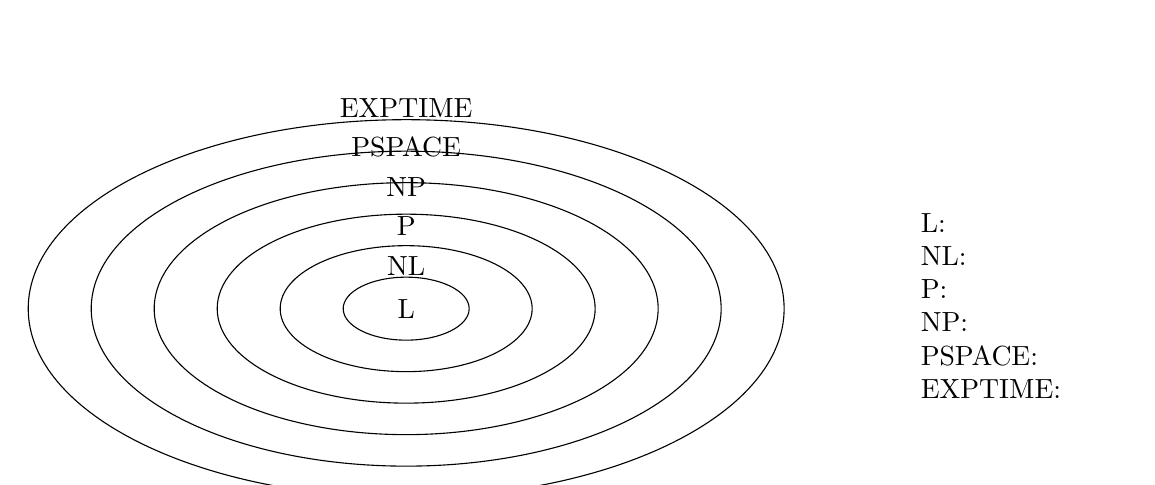
\begin{tikzpicture}[scale=0.8]
        % 绘制复杂性类的包含关系
        \draw (0,0) ellipse (1cm and 0.5cm) node {L};
        \draw (0,0) ellipse (2cm and 1cm) node[above=0.3cm] {NL};
        \draw (0,0) ellipse (3cm and 1.5cm) node[above=0.8cm] {P};
        \draw (0,0) ellipse (4cm and 2cm) node[above=1.3cm] {NP};
        \draw (0,0) ellipse (5cm and 2.5cm) node[above=1.8cm] {PSPACE};
        \draw (0,0) ellipse (6cm and 3cm) node[above=2.3cm] {EXPTIME};
        
        % 添加注释
        \node[right=6.2cm] at (0,0) {
            \begin{tabular}{l}
                L: 对数空间\\
                NL: 非确定性对数空间\\
                P: 多项式时间\\
                NP: 非确定性多项式时间\\
                PSPACE: 多项式空间\\
                EXPTIME: 指数时间
            \end{tabular}
        };
        
        % 添加标题
        \node[above] at (0,3.5) {\large 计算复杂性类的层次结构};
    \end{tikzpicture}
    \caption{复杂性类的包含关系图。每个椭圆代表一个复杂性类,内层的类被外层的类所包含。P=NP问题等价于问第三个和第四个椭圆是否重合。}
    \label{fig:complexity_classes}
\end{figure}

\subsection{近似算法与复杂性}
对于NP-完全等难解问题,我们通常无法在多项式时间内找到精确解,因此需要采用近似算法。近似算法的核心是在合理时间内找到接近最优解的解决方案。近似算法的质量通常用近似比来衡量,即算法解与最优解之比。根据近似比的不同,我们可以将近似算法分为常数比近似(近似比为常数)、对数比近似(近似比与问题规模的对数相关)和多项式比近似(近似比与问题规模的多项式相关)。

更进一步,我们有近似方案的概念。多项式时间近似方案(PTAS)是指对任意$\epsilon > 0$,存在$(1+\epsilon)$近似算法,且其运行时间是输入规模的多项式。而完全多项式时间近似方案(FPTAS)是PTAS的加强版,其运行时间同时关于输入规模和$1/\epsilon$是多项式的。这些近似方案为解决难解问题提供了理论保证,使我们能够在可接受的时间内得到质量有保证的近似解。

\subsection{随机化算法与复杂性}
随机化算法是另一种处理难解问题的重要方法,它通过引入随机性来提高算法的效率或简化算法的设计。随机化算法与确定性算法的主要区别在于,它在执行过程中会使用随机数,因此对于同一输入可能产生不同的输出或具有不同的运行时间。

基于随机化算法的特性,我们定义了一系列随机复杂性类。RP(随机多项式时间)类包含那些存在随机算法的问题,该算法对于"是"的实例至少有1/2的概率给出正确答案,对于"否"的实例总是给出正确答案,且运行时间为多项式。BPP(有界错误概率多项式时间)类则允许算法在两种情况下都有错误,但错误概率不超过1/3。ZPP(零错误概率多项式时间)类是指存在期望运行时间为多项式的随机算法,且该算法总是给出正确答案的问题集合。

随机化算法的主要特点是允许算法使用随机性,可能得到错误结果,但错误概率可控。这种方法在许多情况下能够突破确定性算法的限制,为解决复杂问题提供了新的思路。

\subsection{问题的可计算性}
除了复杂性分类,我们还需要考虑问题是否可计算,这涉及到计算机科学中更加基础的问题。可计算性理论关注的是问题在原则上能否被计算机解决,而不是解决它所需的资源。

\subsubsection{可判定性}
可判定性是指问题是否存在一个算法(图灵机)能够对任意输入实例给出正确答案并且保证停机。可判定问题是指存在图灵机总能给出正确答案且总会停机的问题。这类问题是理论上可以被计算机完全解决的。

相反,不可判定问题是指不存在这样的算法的问题。经典的不可判定问题包括停机问题(判断一个程序是否会在有限时间内终止)、希尔伯特第十问题(判断一个丢番图方程是否有整数解)和后缀问题(判断一个上下文无关语法是否能生成所有可能的字符串)等。这些问题在理论上是无法被任何计算机程序完全解决的,无论计算机多么强大。

\subsubsection{可枚举性}
可枚举性是比可判定性更弱的性质。递归可枚举语言(或称为半可判定问题)是指存在图灵机可以枚举所有属于该语言的字符串的问题集合。对于这类问题,如果一个实例属于该语言,图灵机最终会接受它;但如果不属于,图灵机可能永远不会停机。这意味着我们可以验证"是"的实例,但可能无法确认"否"的实例。

递归语言则是指既是递归可枚举的,其补语言也是递归可枚举的语言。这正好对应于可判定问题。递归语言的特点是存在一个算法可以对任何输入给出明确的"是"或"否"的答案。

\begin{figure}[H]
    \centering
    \begin{tikzpicture}[scale=0.8]
        % 绘制可计算性类的包含关系
        \draw (0,0) ellipse (2cm and 1cm) node {递归语言};
        \draw (0,0) ellipse (4cm and 2cm) node[above=1.3cm] {递归可枚举语言};
        \draw (0,0) ellipse (6cm and 3cm) node[above=2.3cm] {所有语言};
        
        % 添加注释
        \node[right=6.2cm] at (0,0) {
            \begin{tabular}{l}
                递归语言:可判定问题\\
                递归可枚举语言:半可判定问题\\
                所有语言:包括不可判定问题
            \end{tabular}
        };
        
        % 添加标题
        \node[above] at (0,3.5) {\large 可计算性类的层次结构};
    \end{tikzpicture}
    \caption{可计算性类的包含关系图。递归语言是最容易处理的,而有些语言甚至不是递归可枚举的。}
    \label{fig:computability_classes}
\end{figure}

\section{布尔可满足性问题:NP完全性的基石}
布尔可满足性问题(Boolean Satisfiability Problem,简称SAT)是计算机科学中一个具有重要理论和实践意义的问题。它不仅是第一个被证明为NP完全的问题,也是现代许多实际应用中的核心问题。

\subsection{问题的形式化定义}
SAT问题的输入是一个布尔表达式$\varphi$,包含布尔变量$x_1, x_2, \ldots, x_n$,布尔运算符$\neg$ (非),$\wedge$ (与),$\vee$ (或),以及用于指定运算优先级的括号。问题的目标是判定是否存在一个变量赋值,使得表达式$\varphi$的值为真。形式化地,给定布尔函数$\varphi: \{0,1\}^n \rightarrow \{0,1\}$,我们需要判断是否存在$x \in \{0,1\}^n$使得$\varphi(x) = 1$。

\subsection{SAT的标准形式}
SAT问题通常有两种标准形式:合取范式(CNF)和析取范式(DNF)。

合取范式是子句的合取,每个子句是文字的析取。形式上,$\varphi = C_1 \wedge C_2 \wedge \cdots \wedge C_m$,其中每个子句$C_i = l_{i1} \vee l_{i2} \vee \cdots \vee l_{ik}$,每个文字$l_{ij}$是变量或其否定。例如,$(x_1 \vee \neg x_2) \wedge (\neg x_1 \vee x_3) \wedge (x_2 \vee x_3)$是一个CNF公式。

析取范式则是子句的析取,每个子句是文字的合取。形式上,$\varphi = D_1 \vee D_2 \vee \cdots \vee D_m$,其中每个子句$D_i = l_{i1} \wedge l_{i2} \wedge \cdots \wedge l_{ik}$。在DNF中,SAT问题变得容易,因为只需要检查是否存在一个全为真的子句即可。

\subsection{SAT的重要变体}
SAT问题有许多重要变体,其中最著名的是k-SAT和HORN-SAT。

k-SAT是CNF-SAT的特例,其中每个子句恰好包含k个文字。这类问题的复杂性随k的变化而变化:2-SAT是P类问题,有多项式时间算法;而3-SAT及以上是NP完全的。这种差异展示了问题复杂性的微妙变化,仅仅增加一个文字就可能导致问题从易解变为难解。

HORN-SAT是每个子句最多包含一个正文字的CNF公式,可以表示为$(a_1 \wedge a_2 \wedge \cdots \wedge a_k) \rightarrow b$的形式。HORN-SAT是P类问题,可以通过单位传播算法在线性时间内解决。它在逻辑编程和知识表示中有广泛应用。

\begin{figure}[H]
    \centering
    \includegraphics[width=0.9\textwidth]{img/np_reductions.png}
    \caption{NP完全问题之间的归约关系图。图中展示了SAT、3-SAT、图着色、哈密顿回路、TSP等NP完全问题之间的多项式时间归约关系。箭头A→B表示问题A可以归约到问题B,即如果B可以在多项式时间内解决,则A也可以。}
    \label{fig:np_reductions}
\end{figure}

\subsection{SAT的NP完全性证明}
SAT是第一个被证明为NP完全的问题,这一结果由Stephen Cook和Leonid Levin独立证明,因此被称为Cook-Levin定理。证明的核心思想是将任意NP问题的验证过程编码为SAT实例。

证明分为两个部分:首先证明SAT属于NP类,这很简单,因为给定一个变量赋值,我们可以在多项式时间内验证它是否使布尔表达式为真;然后证明所有NP问题都可以多项式时间归约到SAT,这是证明的难点。

归约的基本思路是将验证NP问题解的图灵机执行过程编码为布尔表达式。具体来说,我们为图灵机的每个时间步、每个位置的符号和每个状态创建布尔变量,然后构造布尔表达式来确保这些变量的赋值对应于图灵机的有效计算。这样,图灵机接受当且仅当对应的布尔表达式可满足。

\subsection{SAT求解技术}
由于SAT的理论重要性和实际应用价值,研究人员开发了多种求解技术,大致可分为完备算法和不完备算法。

完备算法保证能找到解(如果存在)或证明不存在解。最基本的完备算法是DPLL(Davis-Putnam-Logemann-Loveland)算法,它基于回溯搜索和单位传播。现代SAT求解器如MiniSAT、Glucose等在DPLL的基础上加入了冲突驱动的子句学习(CDCL)、重启策略、高效的数据结构等技术,能够解决包含数百万变量的实际问题。

不完备算法不保证能找到解或证明无解,但在实践中往往能快速找到解。典型的不完备算法包括局部搜索算法(如WalkSAT)和遗传算法等。这些算法通常用于解决大规模但结构相对简单的SAT实例。

\subsection{SAT的实际应用}
尽管SAT是NP完全问题,但现代SAT求解器的发展使得许多实际应用成为可能:

在硬件验证领域,SAT被用于电路等价性检查、模型检查和测试生成等任务。例如,验证两个电路是否等价可以通过检查它们异或的结果是否恒为假来实现,这可以转化为SAT问题。

在软件验证方面,SAT被用于程序分析、软件测试和漏洞检测等。例如,符号执行技术将程序路径条件编码为SAT实例,通过求解来生成测试用例或检测潜在错误。

在人工智能领域,SAT被用于规划、调度和约束满足问题等。例如,许多约束满足问题可以直接编码为SAT实例,然后使用高效的SAT求解器来解决。

总的来说,SAT问题不仅是计算复杂性理论中的基石,也是连接理论和实践的桥梁,推动了算法设计、软件工具和应用领域的发展。

\subsection{SAT与其他问题的关系}
\subsubsection{规约关系}
\begin{itemize}
    \item \textbf{作为源问题:}
        \begin{itemize}
            \item 许多NP完全问题可以归约到SAT
            \item SAT求解器可以用作通用工具
            \item 归约的效率影响实际应用
        \end{itemize}
    \item \textbf{特殊情况:}
        \begin{itemize}
            \item 某些变体是可解的(如2-SAT)
            \item 存在高效的近似算法
            \item 平均情况分析
        \end{itemize}
\end{itemize}

\subsubsection{理论意义}
\begin{itemize}
    \item \textbf{复杂性理论:}
        \begin{itemize}
            \item NP完全性的基准问题
            \item 复杂性类之间关系的研究
            \item 计算能力的界限探索
        \end{itemize}
    \item \textbf{算法设计:}
        \begin{itemize}
            \item 启发式方法的开发
            \item 近似算法的设计
            \item 参数化复杂性分析
        \end{itemize}
\end{itemize}

\begin{figure}[H]
    \centering
    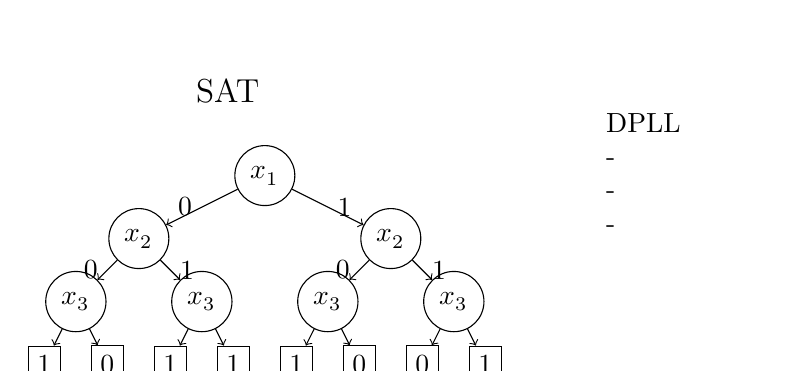
\begin{tikzpicture}[scale=0.8]
        % 绘制SAT求解过程的决策树
        \node[circle,draw] (root) at (0,0) {$x_1$};
        \node[circle,draw] (l1) at (-2,-1) {$x_2$};
        \node[circle,draw] (r1) at (2,-1) {$x_2$};
        \node[circle,draw] (l2) at (-3,-2) {$x_3$};
        \node[circle,draw] (r2) at (-1,-2) {$x_3$};
        \node[circle,draw] (l3) at (1,-2) {$x_3$};
        \node[circle,draw] (r3) at (3,-2) {$x_3$};
        
        % 连接节点
        \draw[->] (root) -- node[left] {0} (l1);
        \draw[->] (root) -- node[right] {1} (r1);
        \draw[->] (l1) -- node[left] {0} (l2);
        \draw[->] (l1) -- node[right] {1} (r2);
        \draw[->] (r1) -- node[left] {0} (l3);
        \draw[->] (r1) -- node[right] {1} (r3);
        
        % 添加结果节点
        \node[rectangle,draw] (res1) at (-3.5,-3) {1};
        \node[rectangle,draw] (res2) at (-2.5,-3) {0};
        \node[rectangle,draw] (res3) at (-1.5,-3) {1};
        \node[rectangle,draw] (res4) at (-0.5,-3) {1};
        \node[rectangle,draw] (res5) at (0.5,-3) {1};
        \node[rectangle,draw] (res6) at (1.5,-3) {0};
        \node[rectangle,draw] (res7) at (2.5,-3) {0};
        \node[rectangle,draw] (res8) at (3.5,-3) {1};
        
        % 连接到结果
        \draw[->] (l2) -- (res1);
        \draw[->] (l2) -- (res2);
        \draw[->] (r2) -- (res3);
        \draw[->] (r2) -- (res4);
        \draw[->] (l3) -- (res5);
        \draw[->] (l3) -- (res6);
        \draw[->] (r3) -- (res7);
        \draw[->] (r3) -- (res8);
        
        % 添加说明
        \node[right=4cm] at (root) {
            \begin{tabular}{l}
                DPLL算法的搜索树:\\
                - 系统地探索所有可能的赋值\\
                - 使用单元传播剪枝\\
                - 冲突驱动的学习
            \end{tabular}
        };
        
        % 添加标题
        \node[above] at (0,1) {\large SAT求解的决策树示例};
    \end{tikzpicture}
    \caption{SAT求解器使用的决策树示例,展示了系统化搜索过程。}
    \label{fig:sat_solver}
\end{figure}

\begin{figure}[H]
    \centering
    \includegraphics[width=0.9\textwidth]{img/sat_example.png}
    \caption{SAT问题的示例及其求解过程。图中展示了一个布尔表达式的合取范式表示,以及DPLL算法在搜索空间中进行系统化探索的决策树。}
    \label{fig:sat_example}
\end{figure}

\section{TSP与SAT问题:NP完全性的桥梁}
旅行商问题(Traveling Salesman Problem,简称TSP)是另一个著名的NP完全问题。通过研究TSP与SAT之间的关系,我们可以更好地理解NP完全性的本质。

\subsection{TSP问题的形式化定义}
TSP问题的输入是一个完全图$G = (V,E)$,其中顶点集$V = \{v_1, v_2, \ldots, v_n\}$代表城市,边权函数$w: E \rightarrow \mathbb{R}^+$表示城市间的距离。问题的目标是找到最短的哈密顿回路,即访问每个顶点恰好一次并返回起点的路径,使总路径长度最小。TSP的判定版本是:给定长度界$L$,判断是否存在长度不超过$L$的哈密顿回路。

\subsection{TSP的变体与特例}
TSP有几个重要的变体和特例。度量TSP要求边权满足三角不等式,即对任意三个顶点$i$、$j$、$k$,有$w(i,j) \leq w(i,k) + w(k,j)$。度量TSP虽然仍是NP完全的,但存在2-近似算法,在实践中更为常见。欧几里得TSP则是顶点在平面上,距离为欧几里得距离的特例,自动满足三角不等式,有更好的近似算法,更接近实际应用场景。

\begin{figure}[H]
    \centering
    \includegraphics[width=0.9\textwidth]{img/tsp_example.png}
    \caption{旅行商问题(TSP)的示例。图中展示了一个完全图,其中顶点代表城市,边权表示城市间的距离,红色路径表示一个可能的最优哈密顿回路。}
    \label{fig:tsp_example}
\end{figure}

\subsection{TSP到SAT的多项式时间归约}
将TSP问题归约到SAT问题是理解NP完全性的重要例子。归约的基本思路是设计布尔变量来表示TSP的解,然后构造布尔表达式来编码TSP的约束条件。

主要使用两类变量:$x_{i,k}$表示城市$i$在位置$k$是否被访问;$y_{i,j}$表示是否直接从城市$i$到城市$j$。基于这些变量,我们构造以下约束条件:

1. 位置唯一性:每个位置恰好访问一个城市,表达式为:
   $\bigwedge_{k=1}^n \left(\bigvee_{i=1}^n x_{i,k}\right) \wedge \bigwedge_{k=1}^n \bigwedge_{i \neq j} (\neg x_{i,k} \vee \neg x_{j,k})$

2. 访问唯一性:每个城市恰好被访问一次,表达式为:
   $\bigwedge_{i=1}^n \left(\bigvee_{k=1}^n x_{i,k}\right) \wedge \bigwedge_{i=1}^n \bigwedge_{k \neq l} (\neg x_{i,k} \vee \neg x_{i,l})$

3. 路径连续性:相邻位置的城市必须有边相连,表达式为:
   $\bigwedge_{k=1}^{n-1} \bigwedge_{i,j=1}^n (x_{i,k} \wedge x_{j,k+1} \rightarrow y_{i,j})$

4. 长度约束:总路径长度不超过界$L$,表达式为:
   $\sum_{i,j=1}^n w_{i,j}y_{i,j} \leq L$

\subsection{归约的复杂性分析}
这个归约的复杂性主要体现在变量和子句的数量上。变量方面,我们有$O(n^2)$个位置变量和$O(n^2)$个边变量,总计$O(n^2)$个变量。子句方面,位置约束和访问约束各需要$O(n^2)$个子句,连续性约束需要$O(n^3)$个子句,长度约束需要$O(n^2)$个子句。因此,整个归约的时间复杂度为$O(n^3)$,是一个多项式时间的归约。

\subsection{求解策略比较}
对于TSP问题,我们可以选择直接求解或通过SAT求解。直接求解TSP的精确算法包括动态规划(时间复杂度$O(n^2 2^n)$)、分支限界(指数时间但有效剪枝)和Held-Karp算法($O(n^2 2^n)$)。也有许多启发式算法,如最近邻居、2-opt局部搜索和蚁群优化等。

通过SAT求解TSP的优点是可以利用成熟的SAT求解器,处理复杂约束,易于添加新约束;缺点是变量和子句数量大,失去问题的几何直观性,可能不如专门的TSP算法高效。

\subsection{两个问题的共同特点}
SAT和TSP问题都具有组合爆炸性,SAT的搜索空间是$2^n$种可能的赋值,TSP是$n!$种可能的路径。两者都具有局部性特征,SAT中变量赋值的局部依赖,TSP中路径的局部优化。在优化技术方面,SAT使用单元传播、学习子句等剪枝策略,TSP使用下界估计、可行性检查;SAT有变量选择策略,TSP有边选择策略。

\begin{figure}[H]
    \centering
    \includegraphics[width=0.9\textwidth]{img/xxx.png}
    \caption{TSP问题归约到SAT问题的示意图,展示了如何将TSP的约束条件转化为布尔表达式。}
    \label{fig:tsp_sat_relation}
\end{figure}

\subsection{实际应用中的选择}
在实际应用中,选择直接求解TSP还是通过SAT求解,需要考虑问题的规模和约束类型。对于小规模问题,两种方法都可行;中等规模问题,专门的TSP算法通常更好;大规模问题则需要启发式方法。如果问题有复杂的附加约束,通过SAT求解可能更为灵活;如果问题结构简单,直接使用TSP算法更为高效。在工业应用中,通常会结合两种方法,利用问题的特殊结构和现有的求解工具。

\subsection{理论意义}
TSP与SAT之间的归约关系具有重要的理论意义。从复杂性理论角度看,这种归约建立了不同问题之间的联系,使我们能够传递复杂性结果,统一问题求解方法。NP完全性的概念帮助我们证明问题的难解性,指导算法设计,启发新的研究方向。从实践角度看,这种关系启示我们思考问题转化的思想,认识通用求解器的价值,以及特殊情况的处理方法。未来的研究方向包括探索新的归约方法、开发混合求解策略,以及探索量子计算在解决这类问题中的应用。

\section{P=NP的影响:计算世界的革命性变革}
P=NP问题的解决,无论是证明它们相等还是不等,都将对计算机科学乃至整个人类社会产生深远的影响。本节将详细探讨这个问题可能的结果及其影响。

\subsection{如果P=NP成立}
\subsubsection{算法设计的革命}
\begin{itemize}
    \item \textbf{效率提升:}
        \begin{itemize}
            \item 所有NP问题都有多项式时间算法
            \item 复杂问题变得"容易"
            \item 计算资源的大幅节省
        \end{itemize}
    \item \textbf{新算法范式:}
        \begin{itemize}
            \item 通用求解策略的出现
            \item 问题转化方法的简化
            \item 算法设计思维的转变
        \end{itemize}
\end{itemize}

\subsubsection{密码学的重构}
\begin{itemize}
    \item \textbf{现有系统的崩溃:}
        \begin{itemize}
            \item RSA等公钥密码系统失效
            \item 数字签名系统需要重建
            \item 安全通信协议需要重设计
        \end{itemize}
    \item \textbf{新方向探索:}
        \begin{itemize}
            \item 基于量子计算的密码系统
            \item 后量子密码学的发展
            \item 新的安全假设的建立
        \end{itemize}
\end{itemize}

\subsubsection{人工智能的飞跃}
\begin{itemize}
    \item \textbf{学习能力:}
        \begin{itemize}
            \item 最优特征选择成为可能
            \item 神经网络训练的优化
            \item 复杂模式的快速识别
        \end{itemize}
    \item \textbf{决策能力:}
        \begin{itemize}
            \item 完美的游戏策略
            \item 优化的资源调度
            \item 精确的风险评估
        \end{itemize}
\end{itemize}

\subsubsection{科学研究的加速}
\begin{itemize}
    \item \textbf{生物信息学:}
        \begin{itemize}
            \item 蛋白质折叠问题的解决
            \item 药物设计的优化
            \item 基因序列分析的突破
        \end{itemize}
    \item \textbf{物理模拟:}
        \begin{itemize}
            \item 量子系统的高效模拟
            \item 材料性质的精确预测
            \item 天气系统的准确建模
        \end{itemize}
\end{itemize}

\subsection{如果P\neq NP成立}
\subsubsection{理论研究的深化}
\begin{itemize}
    \item \textbf{复杂性理论:}
        \begin{itemize}
            \item 复杂性类的精确界定
            \item 中间复杂性类的研究
            \item 近似算法理论的发展
        \end{itemize}
    \item \textbf{算法分析:}
        \begin{itemize}
            \item 下界证明技术的进步
            \item 最优算法的特征研究
            \item 平均情况分析的深入
        \end{itemize}
\end{itemize}

\subsubsection{实践方向的调整}
\begin{itemize}
    \item \textbf{算法设计:}
        \begin{itemize}
            \item 启发式方法的重要性
            \item 近似算法的价值提升
            \item 特殊情况的优化
        \end{itemize}
    \item \textbf{系统架构:}
        \begin{itemize}
            \item 分布式计算的发展
            \item 专用硬件的设计
            \item 混合计算模型的探索
        \end{itemize}
\end{itemize}

\subsection{对各领域的具体影响}
\subsubsection{软件工程}
\begin{itemize}
    \item \textbf{开发过程:}
        \begin{itemize}
            \item 自动化程度提高
            \item 验证和测试的改进
            \item 代码优化的突破
        \end{itemize}
    \item \textbf{软件质量:}
        \begin{itemize}
            \item 错误的自动检测
            \item 性能的精确优化
            \item 安全漏洞的预防
        \end{itemize}
\end{itemize}

\subsubsection{数据科学}
\begin{itemize}
    \item \textbf{数据分析:}
        \begin{itemize}
            \item 复杂模式的发现
            \item 因果关系的推断
            \item 预测模型的优化
        \end{itemize}
    \item \textbf{机器学习:}
        \begin{itemize}
            \item 特征工程的革新
            \item 模型选择的优化
            \item 学习算法的改进
        \end{itemize}
\end{itemize}

\begin{figure}[H]
    \centering
    \includegraphics[width=0.9\textwidth]{img/pnp_impact.png}
    \caption{P=NP问题解决后对各领域的潜在影响示意图,展示了在算法设计、密码学、人工智能和科学研究等领域可能带来的革命性变革。}
    \label{fig:pnp_impact}
\end{figure}

\subsection{社会经济影响}
\subsubsection{经济结构}
\begin{itemize}
    \item \textbf{产业变革:}
        \begin{itemize}
            \item 传统行业的自动化
            \item 新兴产业的出现
            \item 就业结构的改变
        \end{itemize}
    \item \textbf{市场效率:}
        \begin{itemize}
            \item 资源配置的优化
            \item 市场预测的准确性
            \item 金融系统的重构
        \end{itemize}
\end{itemize}

\subsubsection{社会发展}
\begin{itemize}
    \item \textbf{教育变革:}
        \begin{itemize}
            \item 学习方式的改变
            \item 知识获取的效率
            \item 教育资源的分配
        \end{itemize}
    \item \textbf{医疗进步:}
        \begin{itemize}
            \item 疾病诊断的准确性
            \item 药物研发的加速
            \item 医疗资源的优化
        \end{itemize}
\end{itemize}

\subsection{伦理与安全考虑}
\subsubsection{隐私保护}
\begin{itemize}
    \item \textbf{数据安全:}
        \begin{itemize}
            \item 加密方案的重构
            \item 隐私保护的新方法
            \item 安全协议的改变
        \end{itemize}
    \item \textbf{社会影响:}
        \begin{itemize}
            \item 个人隐私的界定
            \item 数据使用的规范
            \item 法律框架的调整
        \end{itemize}
\end{itemize}

\subsubsection{权力平衡}
\begin{itemize}
    \item \textbf{技术垄断:}
        \begin{itemize}
            \item 计算能力的集中
            \item 资源分配的失衡
            \item 技术差距的扩大
        \end{itemize}
    \item \textbf{社会控制:}
        \begin{itemize}
            \item 监控能力的提升
            \item 决策权的集中
            \item 自由度的减少
        \end{itemize}
\end{itemize}

\begin{figure}[H]
    \centering
    \begin{tikzpicture}[scale=0.8]
        % 创建时间轴
        \draw[->,thick] (-6,0) -- (6,0);
        \node[right] at (6,0) {时间};
        
        % 添加关键时间点
        \node[circle,fill=black,inner sep=2pt] (now) at (0,0) {};
        \node[above] at (0,0.3) {P=NP解决};
        
        % 添加影响阶段
        \node[rectangle,draw,fill=lightgray] at (-4,4) {当前阶段};
        \node[rectangle,draw,fill=lightgray] at (0,4) {过渡期};
        \node[rectangle,draw,fill=lightgray] at (4,4) {新范式};
        
        % 添加影响描述
        \node[align=left] at (-4,2) {
            \begin{tabular}{l}
                - 算法优化\\
                - 启发式方法\\
                - 近似解决方案
            \end{tabular}
        };
        
        \node[align=left] at (0,2) {
            \begin{tabular}{l}
                - 系统重构\\
                - 标准更新\\
                - 方法转变
            \end{tabular}
        };
        
        \node[align=left] at (4,2) {
            \begin{tabular}{l}
                - 新技术范式\\
                - 社会重组\\
                - 新机遇出现
            \end{tabular}
        };
        
        % 添加连接线
        \draw[dashed] (-4,1.5) -- (-2,0.1);
        \draw[dashed] (0,1.5) -- (0,0.1);
        \draw[dashed] (4,1.5) -- (2,0.1);
    \end{tikzpicture}
    \caption{P=NP问题解决后的发展时间线示意图。}
    \label{fig:pnp_timeline}
\end{figure}

\subsection{未来展望}
\subsubsection{技术发展}
\begin{itemize}
    \item \textbf{新计算模型:}
        \begin{itemize}
            \item 量子计算的发展
            \item 生物计算的探索
            \item 混合计算系统
        \end{itemize}
    \item \textbf{应用创新:}
        \begin{itemize}
            \item 智能系统的进步
            \item 自动化水平的提高
            \item 新型应用的出现
        \end{itemize}
\end{itemize}

\subsubsection{理论研究}
\begin{itemize}
    \item \textbf{新问题探索:}
        \begin{itemize}
            \item 后P=NP时代的理论
            \item 新的复杂性度量
            \item 计算模型的扩展
        \end{itemize}
    \item \textbf{跨学科融合:}
        \begin{itemize}
            \item 与物理学的结合
            \item 与生物学的交叉
            \item 与认知科学的融合
        \end{itemize}
\end{itemize}

\begin{figure}[H]
    \centering
    \begin{tikzpicture}[scale=0.8]
        % 创建两种情况的对比图
        \node[rectangle,draw,minimum width=5cm,minimum height=3cm] (peq) at (-3,0) {
            \begin{tabular}{c}
                P = NP\\
                \hline
                算法革命\\
                安全重构\\
                效率提升\\
                社会变革
            \end{tabular}
        };
        
        \node[rectangle,draw,minimum width=5cm,minimum height=3cm] (pneq) at (3,0) {
            \begin{tabular}{c}
                P $\neq$ NP\\
                \hline
                理论深化\\
                方法优化\\
                专业分化\\
                渐进发展
            \end{tabular}
        };
        
        % 添加比较箭头
        \draw[<->] (peq) -- node[above] {影响对比} (pneq);
        
        % 添加说明
        \node[below=2cm] at (0,0) {
            \begin{tabular}{c}
                两种结果的影响比较:\\
                - 发展速度\\
                - 变革程度\\
                - 社会影响\\
                - 技术路线
            \end{tabular}
        };
    \end{tikzpicture}
    \caption{P=NP问题两种可能结果的影响对比。}
    \label{fig:pnp_comparison}
\end{figure}

\section{结论}
P vs NP问题作为计算机科学中最重要的未解决问题之一,其重要性和影响力远超出了理论计算机科学的范畴。通过本报告的研究,我们可以得出以下结论:

\subsection{理论意义}
\begin{itemize}
    \item \textbf{计算理论的基石:}
        \begin{itemize}
            \item 定义了计算复杂性的本质
            \item 建立了问题难度的度量标准
            \item 推动了算法设计的发展
        \end{itemize}
    \item \textbf{数学价值:}
        \begin{itemize}
            \item 连接了多个数学分支
            \item 启发了新的研究方法
            \item 提供了重要的研究工具
        \end{itemize}
\end{itemize}

\subsection{实践价值}
\begin{itemize}
    \item \textbf{算法设计:}
        \begin{itemize}
            \item 指导了效率优化方向
            \item 促进了近似算法发展
            \item 推动了启发式方法研究
        \end{itemize}
    \item \textbf{应用发展:}
        \begin{itemize}
            \item 影响密码学设计
            \item 推动人工智能进步
            \item 促进跨学科应用
        \end{itemize}
\end{itemize}

\subsection{研究现状}
\begin{itemize}
    \item \textbf{主要进展:}
        \begin{itemize}
            \item 相关问题的深入研究
            \item 新的证明方法探索
            \item 复杂性类的细化
        \end{itemize}
    \item \textbf{存在挑战:}
        \begin{itemize}
            \item 证明技术的局限性
            \item 问题本质的深度
            \item 研究方法的创新需求
        \end{itemize}
\end{itemize}

\subsection{未来展望}
\begin{itemize}
    \item \textbf{研究方向:}
        \begin{itemize}
            \item 新的证明技术探索
            \item 量子计算的应用
            \item 跨学科方法的融合
        \end{itemize}
    \item \textbf{应用前景:}
        \begin{itemize}
            \item 算法效率的提升
            \item 新型计算模型的发展
            \item 实际应用的拓展
        \end{itemize}
\end{itemize}

\begin{figure}[H]
    \centering
    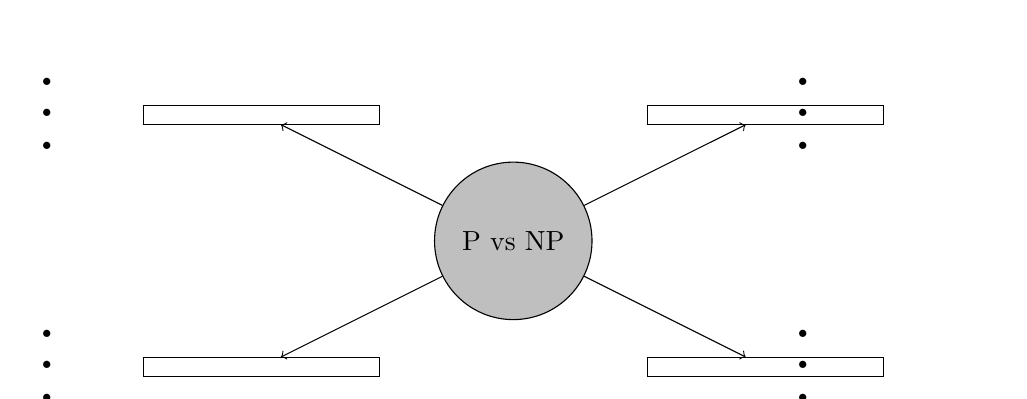
\begin{tikzpicture}[scale=0.8]
        % 创建中心节点
        \node[circle,draw,fill=lightgray,minimum size=2cm] (center) at (0,0) {P vs NP};
        
        % 创建四个主要方面
        \node[rectangle,draw,minimum width=3cm] (theory) at (-4,2) {理论意义};
        \node[rectangle,draw,minimum width=3cm] (practice) at (4,2) {实践价值};
        \node[rectangle,draw,minimum width=3cm] (status) at (-4,-2) {研究现状};
        \node[rectangle,draw,minimum width=3cm] (future) at (4,-2) {未来展望};
        
        % 添加连接线
        \draw[->] (center) -- (theory);
        \draw[->] (center) -- (practice);
        \draw[->] (center) -- (status);
        \draw[->] (center) -- (future);
        
        % 添加子项
        \node[text width=2.5cm,align=left] at (-6,2) {
            \small
            • 复杂性理论\\
            • 算法设计\\
            • 数学基础
        };
        
        \node[text width=2.5cm,align=left] at (6,2) {
            \small
            • 效率优化\\
            • 应用发展\\
            • 技术创新
        };
        
        \node[text width=2.5cm,align=left] at (-6,-2) {
            \small
            • 主要进展\\
            • 现有方法\\
            • 关键挑战
        };
        
        \node[text width=2.5cm,align=left] at (6,-2) {
            \small
            • 研究方向\\
            • 应用前景\\
            • 发展趋势
        };
    \end{tikzpicture}
    \caption{P vs NP问题研究的主要方面总结。}
    \label{fig:conclusion_summary}
\end{figure}

\subsection{个人思考}
通过对P vs NP问题的深入研究,我认为:
\begin{itemize}
    \item \textbf{问题的本质:}
        \begin{itemize}
            \item 反映了计算与智能的深层关系
            \item 揭示了问题求解的普遍规律
            \item 体现了科学探索的哲学意义
        \end{itemize}
    \item \textbf{研究的价值:}
        \begin{itemize}
            \item 推动了计算理论的发展
            \item 促进了跨学科的交流
            \item 启发了新的研究思路
        \end{itemize}
    \item \textbf{未来的期望:}
        \begin{itemize}
            \item 继续探索新的研究方法
            \item 关注实际应用的发展
            \item 保持开放创新的态度
        \end{itemize}
\end{itemize}

\begin{figure}[H]
    \centering
    \begin{tikzpicture}[scale=0.8]
        % 创建时间轴
        \draw[->,thick] (-6,0) -- (6,0);
        \node[right] at (6,0) {发展历程};
        
        % 添加关键节点
        \node[circle,fill=black,inner sep=2pt] (past) at (-4,0) {};
        \node[circle,fill=black,inner sep=2pt] (present) at (0,0) {};
        \node[circle,fill=black,inner sep=2pt] (future) at (4,0) {};
        
        % 添加标签
        \node[above] at (-4,0.3) {问题提出};
        \node[above] at (0,0.3) {当前研究};
        \node[above] at (4,0.3) {未来发展};
        
        % 添加描述
        \node[below,text width=3cm,align=center] at (-4,-0.5) {
            \small
            • 理论基础\\
            • 初步研究\\
            • 基本框架
        };
        
        \node[below,text width=3cm,align=center] at (0,-0.5) {
            \small
            • 深入探索\\
            • 方法创新\\
            • 应用拓展
        };
        
        \node[below,text width=3cm,align=center] at (4,-0.5) {
            \small
            • 新技术应用\\
            • 跨学科融合\\
            • 理论突破
        };
    \end{tikzpicture}
    \caption{P vs NP问题研究的发展历程与展望。}
    \label{fig:research_timeline}
\end{figure}

总的来说,P vs NP问题不仅是一个数学问题或计算机科学问题,更是一个关于人类认知能力和问题求解本质的深层次探讨。无论这个问题最终被证明为P=NP还是P$\neq$NP,研究过程本身已经极大地推动了计算机科学的发展,并将继续影响着未来的科技进步。在未来的研究中,我们应该保持开放的思维,积极探索新的研究方法和应用方向,为这个重要问题的解决做出贡献。

\begin{figure}[H]
    \centering
    \includegraphics[width=0.9\textwidth]{img/pnp_relation.png}
    \caption{P、NP和NP完全问题之间的关系总结图。此图展示了三个复杂性类的包含关系,以及P=NP问题的核心——如果P=NP成立,则三者完全重合;如果P≠NP成立,则P是NP的真子集。}
    \label{fig:pnp_relation}
\end{figure}

\begin{figure}[H]
    \centering
    \includegraphics[width=0.9\textwidth]{img/complexity_hierarchy.png}
    \caption{复杂性类的包含关系图。展示了从AC0到EXPSPACE的主要复杂性类之间的包含关系,以及每个类中的典型问题。P=NP问题是计算机科学中最重要的未解决问题之一,它询问P类和NP类是否相等。}
    \label{fig:complexity_classes}
\end{figure}

\section{参考文献}
\begin{thebibliography}{99}

\bibitem{cook1971complexity}
Cook, S. A. (1971).
\textit{The complexity of theorem-proving procedures}.
In Proceedings of the third annual ACM symposium on Theory of computing (pp. 151-158).
ACM.

\bibitem{karp1972reducibility}
Karp, R. M. (1972).
\textit{Reducibility among combinatorial problems}.
In Complexity of computer computations (pp. 85-103).
Springer.

\bibitem{levin1973universal}
Levin, L. A. (1973).
\textit{Universal sequential search problems}.
Problems of Information Transmission, 9(3), 265-266.

\bibitem{garey1979computers}
Garey, M. R., \& Johnson, D. S. (1979).
\textit{Computers and intractability: A guide to the theory of NP-completeness}.
W. H. Freeman.

\bibitem{sipser2006introduction}
Sipser, M. (2006).
\textit{Introduction to the Theory of Computation}.
Course Technology.

\bibitem{arora2009computational}
Arora, S., \& Barak, B. (2009).
\textit{Computational complexity: a modern approach}.
Cambridge University Press.

\bibitem{goldreich2010p}
Goldreich, O. (2010).
\textit{P, NP, and NP-Completeness: The basics of computational complexity}.
Cambridge University Press.

\bibitem{aaronson2016p}
Aaronson, S. (2017).
\textit{P =? NP}.
In J. F. Nash Jr. \& M. Th. Rassias (Eds.), Open Problems in Mathematics (pp. 1-122).
Springer, Cham.

\bibitem{wigderson2019mathematics}
Wigderson, A. (2019).
\textit{Mathematics and Computation: A Theory Revolutionizing Technology and Science}.
Princeton University Press.

\bibitem{fortnow2013golden}
Fortnow, L. (2013).
\textit{The Golden Ticket: P, NP, and the Search for the Impossible}.
Princeton University Press.

\bibitem{papadimitriou1994computational}
Papadimitriou, C. H. (1994).
\textit{Computational complexity}.
Addison-Wesley.

\bibitem{hopcroft2001introduction}
Hopcroft, J. E., Motwani, R., \& Ullman, J. D. (2001).
\textit{Introduction to automata theory, languages, and computation}.
Addison-Wesley.

\bibitem{dasgupta2008algorithms}
Dasgupta, S., Papadimitriou, C. H., \& Vazirani, U. V. (2008).
\textit{Algorithms}.
McGraw-Hill.

\bibitem{kleinberg2006algorithm}
Kleinberg, J., \& Tardos, É. (2006).
\textit{Algorithm design}.
Pearson Education.

\bibitem{cormen2009introduction}
Cormen, T. H., Leiserson, C. E., Rivest, R. L., \& Stein, C. (2009).
\textit{Introduction to algorithms}.
MIT press.

\bibitem{impagliazzo2001complexity}
Impagliazzo, R. (2001).
\textit{A personal view of average-case complexity}.
In Proceedings 16th Annual IEEE Conference on Computational Complexity (pp. 134-147).
IEEE.

\bibitem{razborov1994natural}
Razborov, A. A., \& Rudich, S. (1994).
\textit{Natural proofs}.
In Proceedings of the twenty-sixth annual ACM symposium on Theory of computing (pp. 204-213).
ACM.

\bibitem{williams2014algorithms}
Williams, R. (2014).
\textit{Algorithms for circuits and circuits for algorithms}.
In Proceedings of the 29th Annual IEEE Conference on Computational Complexity (pp. 21-32).
IEEE.

\bibitem{babai2016graph}
Babai, L. (2016).
\textit{Graph isomorphism in quasipolynomial time}.
In Proceedings of the forty-eighth annual ACM symposium on Theory of Computing (pp. 684-697).
ACM.

\bibitem{dinur2007pcp}
Dinur, I. (2007).
\textit{The PCP theorem by gap amplification}.
Journal of the ACM (JACM), 54(3), Article 12.

\bibitem{valiant1979complexity}
Valiant, L. G. (1979).
\textit{The complexity of computing the permanent}.
Theoretical computer science, 8(2), 189-201.

\bibitem{razborov1985lower}
Razborov, A. A. (1985).
\textit{Lower bounds on the monotone complexity of some Boolean functions}.
In Soviet Mathematics Doklady (Vol. 31, pp. 354-357).

\bibitem{mulmuley2001geometric}
Mulmuley, K. D., \& Sohoni, M. (2001).
\textit{Geometric complexity theory I: An approach to the P vs. NP and related problems}.
SIAM Journal on Computing, 31(2), 496-526.

\bibitem{agrawal2004primes}
Agrawal, M., Kayal, N., \& Saxena, N. (2004).
\textit{PRIMES is in P}.
Annals of Mathematics, 160(2), 781-793.

\bibitem{khot2002power}
Khot, S. (2002).
\textit{On the power of unique 2-prover 1-round games}.
In Proceedings of the thiry-fourth annual ACM symposium on Theory of computing (pp. 767-775).
ACM.

\end{thebibliography}



\end{document}
ACM.

\end{thebibliography}



\end{document}